\documentclass[a4paper,dvipdfmx,11pt]{jsreport}


% 数式
\usepackage{amsmath,amsfonts}
\usepackage{bm}
\usepackage{listings,plistings}
\usepackage{url}
\usepackage{courier}
\usepackage[top=20truemm,bottom=20truemm,left=25truemm,right=25truemm]{geometry}
\lstset{
   basicstyle={\ttfamily\small},
   frame=tRBl,
   framesep=10pt,
   breaklines=true,
   linewidth=17.5cm,
    lineskip=-0.5ex,
    tabsize=2,
	basewidth={0.65em,0.65em},
	language=Python,
}
% 画像
\usepackage[dvipdfmx]{graphicx}
\usepackage{here}
\usepackage{pdfpages} 
\usepackage{physics}

\usepackage{multicol}
\usepackage{moreverb}


\setlength{\columnsep}{4.5cm}

\begin{document}

\title{データベースシステムI\\最終レポート課題}
\author{筑波大学 情報学群 情報メディア創成学類 3年\\ 2022***** 田村 匠}
\date{\today}
\maketitle

\tableofcontents

\chapter{目的}
\section{はじめに}
今回の最終レポート課題では,私は「親父ギャクコロシアム」という
親父ギャグの投稿・評価が行えるWebアプリを作成した.

私は親父ギャクが大好きで,日常生活の中で思い付き,
発言してしまうことも多い.
その場合,多くは「寒い」「つまらない」といった評価をいただくことになる.
しかしながら,まれに「面白い」という評価をいただくこともある.

同じ親父ギャクにもかかわらず,面白さと寒さにギャグが分類されるのはなぜだろうか.
どのようにすれば,面白い親父ギャクのエッセンスを得ることができるだろうか.

そこで,私は親父ギャクを投稿し,「面白い」「寒い」の両軸で評価できる
「親父ギャクコロシアム」というWebサービスを開発することを思いついた.

親父ギャクを集積し,ユーザーが評価を行うことで,面白い,あるいは寒いギャグのデータがたまり,
将来的には,その傾向を分析することができるようになるだろう.

\section{関連事例}
「親父ギャクコロシアム」のコンセプトと類似する既存Webサービスとしては,
ダジャレ・ステーション\cite{dajare-sta}が挙げられる.

ダジャレ・ステーションはダジャレを投稿し,評価・検索できるサービスである.
しかしながら,ダジャレ・ステーションと「親父ギャクコロシアム」には以下の違いがある.

\begin{itemize}
  \item 「ダジャレ」ではなく「親父ギャク」である.
  \item ダジャレ・ステーションは面白さのみを評価するが,親父ギャクには「面白い」と「寒い」の2つの評価軸が必要である.
\end{itemize}

また,何かを投稿し,評価するという概念は,一般的なSNSの概念と一致している.
一般的にこのようなサイトは,アカウント作成を経て,投稿・評価を行う.
また,このようなサイトは機能の追加削除が柔軟に行われる傾向がある.
そのため,データベース設計においては,機能の追加削除を容易に行える設計も
重要になるだろう.

今回の課題においては,このような先行事例を踏まえつつ,
データベースの設計・活用を主眼に置きながら,Webアプリの開発を行った.

\section{実装方法と制約事項}
サービスは,講義資料で示された通りに筑波大学のイントラネット内に構築した.
PythonとFlaskを用い,開発を行った.
データベースシステムとしてはMySQLとmongoDBを利用し,これらは
講義で用意されたホストを用いた.

開発にあたっては,実際にWebアプリを公開することが目的ではなく,
RDBMSあるいは,NoSQLデータベースシステムに関する理解を深めることが
目的であることを考慮し,機能・デザイン面においては最低限の実装のみを行った.

また,セキュリティの面においては,データベースシステムと密接にかかわる
SQLインジェクションなどに関しては重点的に対策を行ったが,
CSRF攻撃やログイン機能に対するブルートフォース攻撃などへの対策は完璧ではない状態となっている.

最後にWebアプリのシステムは大量のデータを処理することを現時点では想定していない.
何十万ものアクセスや投稿があった場合,システムは正常に動作しない.

システムの起動は,以下のコマンドで行う.
\begin{lstlisting}
$ python app.py
\end{lstlisting}
サイトは,\url{http://localhost:11067/}にホストされる.
\chapter{説明}
\section{機能説明・スクリーンショット}
親父ギャクコロシアムの機能は主に,以下の3つで説明される.
\begin{enumerate}
  \item ユーザー認証(セッション管理)
  \item 親父ギャグの投稿
  \item 親父ギャグの閲覧・評価
\end{enumerate}
この節では,各機能について,スクリーンショットを提示しながら,機能を説明する.

サイトは,\url{http://localhost:11067/}にホストされ,
トップページは図\ref{fig:top_unauth}のようになっている.

\begin{figure}[tb]
  \centering
  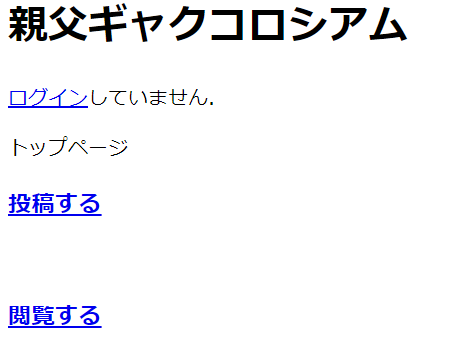
\includegraphics[width=8cm]{img/top_unauth.png}
  \caption{未ログイン状態のトップページ\label{fig:top_unauth}}
\end{figure}

\subsection{ユーザー認証}
閲覧機能以外はログインをしなければ,利用することができない.
未ログインの状態で,図\ref{fig:top_unauth}の「投稿する」などを押した場合,
警告メッセージとともに,図\ref{fig:login_post}のようなログイン画面に遷移する.
\begin{figure}[tb]
  \centering
  \includegraphics*[width=13cm]{img/login_post.png}
  \caption{ログインを促すメッセージ付きのログイン画面 \label{fig:login_post}}
\end{figure}

今回は,アカウントを作成していないため,「ここから登録できます.」を
クリックして,アカウントを作成する.
図\ref{fig:register}のように,登録画面でアカウントを作成する.
\begin{figure}[tb]
  \centering
  \includegraphics*[width=13cm]{img/register.png}
  \caption{アカウント登録画面\label{fig:register}}
\end{figure}

アカウント作成時には,
\begin{itemize}
  \item ユーザIDは半角英数字とアンダーバーのみ利用でる.
  \item パスワードは5文字以上50文字以内で設定する.
\end{itemize}
というルールがあり,ルールを満たしていない場合は,
その旨が警告され,アカウント作成はできない.

アカウントを作成すると,
図\ref{fig:top_auth}のように,ログイン状態で,
トップページに戻る.
\begin{figure}[tb]
  \centering
  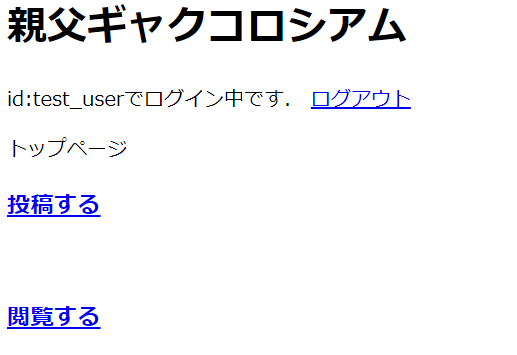
\includegraphics[width=8cm]{img/top_auth.png}
  \caption{ログイン状態のトップページ\label{fig:top_auth}}
\end{figure}

「ログアウト」を行い,「ログイン」から今設定した
ユーザID・パスワードでログインすることはもちろん可能である.

\subsection{親父ギャクの投稿}
ログイン状態の場合,投稿が可能である.
トップページの「投稿する」から図\ref{fig:post}の
投稿画面に遷移できる.
\begin{figure}[tb]
  \centering
  \includegraphics*[width=14cm]{img/post.png}
  \caption{投稿画面\label{fig:post}}
\end{figure}
「投稿」を押すと,図\ref{fig:post_confirm}の投稿確認画面へ遷移する.
ここで内容を確認し,前の画面に戻り修正することができる.
\begin{figure}[tb]
  \centering
  \includegraphics*[width=13cm]{img/post_confirm.png}
  \caption{投稿確認画面\label{fig:post_confirm}}
\end{figure}
問題がなければ,「投稿」を押す.すると,トップページに戻る.

\subsection{親父ギャグの閲覧・評価}
トップページから「閲覧する」をクリックすると,
図\ref{fig:view}のように,
投稿されたギャグを確認できる.
\begin{figure}[tb]
  \centering
  \includegraphics*[width=15cm]{img/view.png}
  \caption{閲覧・評価画面(寒い順でソートした場合)\label{fig:view}}
\end{figure}

ログイン状態であれば,面白い,あるいは,寒いの評価を
絵文字を押すことで行うことができる.
1度絵文字を押すと,絵文字は表示されなくなる.
1ユーザー1評価が原則となっている.

評価の数や投稿時間で,並び替えを行うことができる.

\section{使用したデータベースとデータベース設計}

\renewcommand{\bibname}{参考文献}
\bibliographystyle{jplain}
\bibliography{bibtex}

\end{document}